\documentclass[week2]{csse1001}

\title{CSSE1001 Week 5 Practicals}
 
\begin{document}

\begin{frame} 
\maketitle
\end{frame}

\section{Some assignment dos and don'ts...}

\begin{topic}{Bad: Global variables}
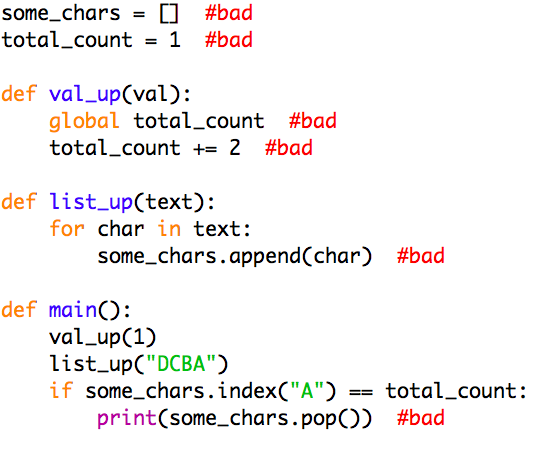
\includegraphics[scale=1]{bad_python/globals}
\end{topic}

\begin{topic}{Good: Use of constants}
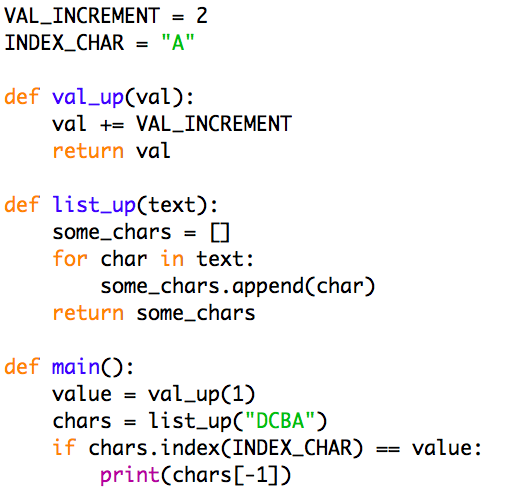
\includegraphics[scale=1]{bad_python/constants}
\end{topic}

\begin{topic}{Bad: Lazy variable naming}
\includegraphics[scale=1]{bad\_python/bad\_naming}
\end{topic}

\begin{topic}{Good: Meaningful variable names}
\includegraphics[scale=1]{bad\_python/good\_naming}
\end{topic}

\begin{topic}{Bad: Lengthy functions}
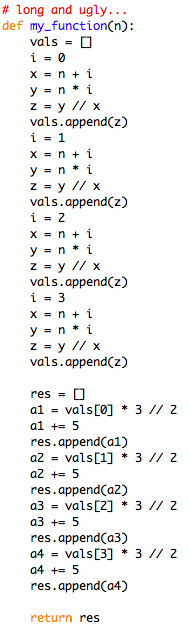
\includegraphics[scale=1]{bad\_python/long}
\end{topic}

\begin{topic}{Good: Functional decomposition and good use of control structures}
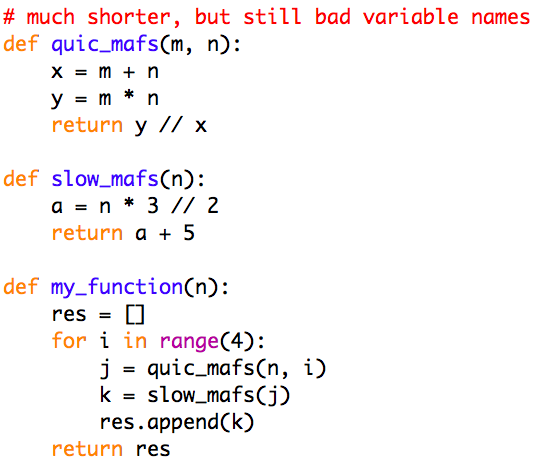
\includegraphics[scale=1]{bad\_python/short}
\end{topic}

\begin{topic}{Bad: Not following the spec}
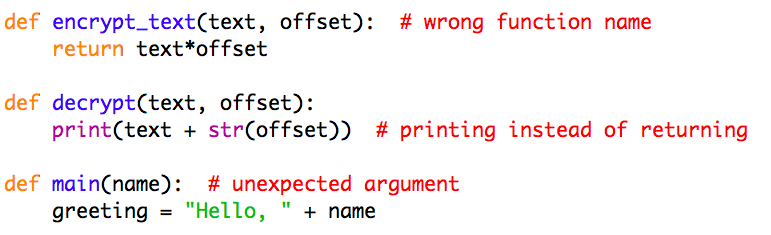
\includegraphics[scale=1]{bad\_python/incorrect}
(note that the implementations are completely absurd...)
\end{topic}

\begin{topic}{Good: Following the spec exactly}
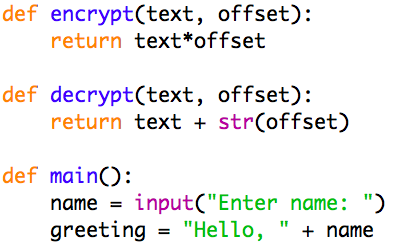
\includegraphics[scale=1]{bad\_python/correct}
(note that the implementations are completely absurd...)
\end{topic}

\begin{topic}{Bad: No documentation}
\includegraphics[scale=1]{bad\_python/no\_comments}
\end{topic}

\begin{topic}{Also Bad: Overcommenting}
\includegraphics[scale=1]{bad\_python/bad\_comments}
\end{topic}

\begin{topic}{Good: Appropriate docstrings and comments}
\includegraphics[scale=1]{bad\_python/good\_comments}
\end{topic}

\section{Sample tests}

\end{document} 
